%
\section{Apprendimento supervisionato}
\label{sec:apprendimento supervisionato}
In questa sezione viene portata avanti una descrizione più approfondita e formale dell'apprendimento supervisionato.\\
Come già accennato precedentemente, quando si parla di apprendimento supervisionato si hanno a disposizione sia gli input \textbf{x} che i corrispettivi target di output \textbf{y}; esisterà quindi una funzione 
\textbf{y} = f(\textbf{x}) che mette in relazione gli input con gli output. Tuttavia, come detto, tale funzione è incognita ed è quindi ciò che viene ricercato con l'algoritmo di apprendimento.
Nella pratica si cerca di approssimare la funzione agendo su una serie di parametri $\bm{\theta}$, quindi si avrà un qualcosa del tipo: \textbf{y'} = f'(\textbf{x},$\bm{\theta}$). \\

\begin{figure}[h!]
	\centering
	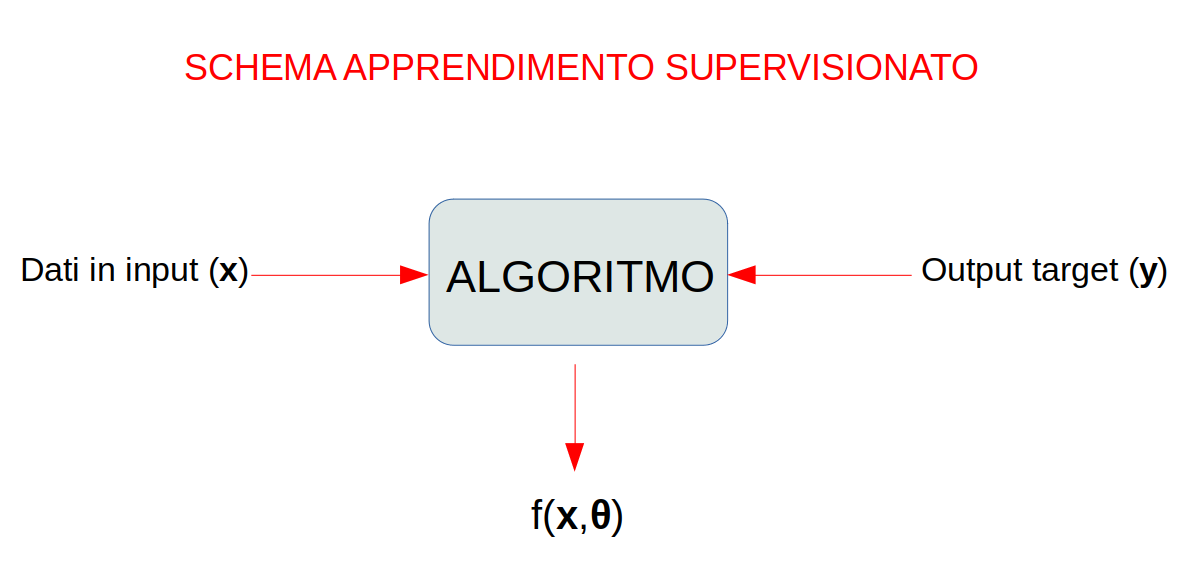
\includegraphics[width=0.85\textwidth]{figs/App_sup.png}
	\caption{si riporta uno schema intuitivo del funzionamento di un algoritmo di apprendimento supervisionato}
	\label{fig:schema_app_sup}
\end{figure}


Per ogni vettore \textbf{x} del training data set è possibile definire una particolare funzione detta "Loss function" L(\textbf{y},f(\textbf{x},$\bm{\theta}$)); a questo punto è possibile fare una media della funzione di perdita sull'intero set di dati a disposizione, ottenendo la funzione di rischio: \\
\begin{equation}
	R(\bm{\theta}) = \frac{1}{N}\sum_{k=1}^{N}L(\textbf{y},f(\textbf{x},\bm{\theta}))
\end{equation}
dove N è il numero di eventi del training data set. \\
Un esempio di funzione di rischio molto diffusa è l'errore quadratico medio:
\begin{equation}
	R(\bm{\theta}) = \frac{1}{N}\sum_{k=1}^{N}(\textbf{y}_k - f(\textbf{x}_k , \bm{\theta}))^2
\end{equation}
Quando si addestra un modello si vuole inoltre evitare il così detto overfitting, ovvero il fatto che il modello si è adattato troppo bene ai dati del training data set, non raggiungendo la generalità richiesta. Un modo per verificare un eventuale overfitting è quello di verificare se il modello è nettamente migliore per il data set di allenamento rispetto al data set di test. \\
Per arginare questo problema è possibile modificare la funzione di rischio, definendo la funzione di costo:
\begin{equation}
	C(\bm{\theta}) = R(\bm{\theta}) + \lambda Q(\bm{\theta})
\end{equation}
con $\lambda$ parametro.
A questo punto l'obiettivo è quello di minimizzare la funzione di rischio (o di costo in caso di overfitting) e per fare ciò esistono diversi metodi, fra i quali il più comune è il metodo di discesa del gradiente.

\newpage

\subsection{Discesa del gradiente}
\label{discesa del gradiente}
La discesa del gradiente è una tecnica di ottimizzazione utilizzata per minimizzare l'errore che si introduce stimando la \textbf{y'} = f'(\textbf{x},$\bm{\theta}$) rispetto alla funzione "vera" \textbf{y} = f(\textbf{x}). \\
Si consideri quindi una Loss function L(\textbf{y},f(\textbf{x},$\bm{\theta}$)) ed un vettore dei parametri $\bm{\theta}$ con i quali è possibile calcolare: \\
\begin{equation}
	\textbf{G} = \frac{1}{N} \sum_{k=1}^{N} \boldsymbol{\nabla}_\theta L(\textbf{y},f(\textbf{x},\bm{\theta})) 
\end{equation} 
Una volta calcolato \textbf{G} è possibile aggiornare il vettore dei parametri $\bm{\theta}$ nel modo seguente:
\begin{equation}
\bm{\theta} - \epsilon\textbf{G} \rightarrow \bm{\theta}
\end{equation}
Qui $\epsilon$ prende il nome di passo ed ha il ruolo di calibrare di quanto debba essere modificato il vettore \bm{$\theta$} nella direzione opposta a quella del gradiente \textbf{G}.\\
Per completezza si riporta il fatto che, quando si ha un elevato campione nel training data set, si utilizza il metodo di discesa del gradiente stocastico, che è strutturato allo stesso modo di quello appena descritto ma viene limitato ad un sottoinsieme del data set di allenamento per una questione di lunghezza di calcolo.\\

%
